%\documentclass[pdftex,12pt,a4paper]{article}
\documentclass[10pt]{article}

\usepackage[left=2.5cm,top=2.5cm,bottom=2.5cm,right=2.5cm]{geometry}


\usepackage[utf8]{inputenc}
%\usepackage[T1]{fontenc}
\usepackage[spanish]{babel}
\usepackage{amssymb,amsmath,amsthm}
\usepackage{fancyhdr}
\usepackage{bm}
\usepackage{graphics}
\usepackage{graphicx}
\usepackage{caption}
\usepackage{subfig}
\usepackage{setspace}
\usepackage{natbib}
\usepackage{float}

%%para ecuaciones$$$
\usepackage{listings}

\lstdefinestyle{PY}{
language = Python,
frame = single,
keywordstyle = \color{blue},
commentstyle=\color{red},
basicstyle = \footnotesize \ttfamily,
breaklines=true,
showstringspaces=false            % importante para python
}

\lstdefinestyle{as}{
language = Python,
keywordstyle = \color{blue},
commentstyle=\color{red},
basicstyle = \footnotesize \ttfamily,
breaklines=true,
showstringspaces=false            % importante para python
}
%%%%%%%%%%%%%%%%%%%%%%%%


\usepackage{tikz}
\def\checkmark{\tikz\fill[scale=0.4](0,.35) -- (.25,0) -- (1,.7) -- (.25,.15) -- cycle;}



\newcommand{\HRule}{\rule{\linewidth}{0.25mm}}
\newcommand{\floor}[1]{\lfloor #1 \rfloor}



%%%%%%%%comienza documento%%%%%%%%%%
\begin{document}

%%%%%%%%PORTADA%%%%%
\begin{center}

\includegraphics[width=0.2\textwidth]{images/logo_usm}~\\[1.2cm]
~\\[-1.5cm]

\textsc{\large Universidad T\'ecnica Federico Santa Mar\'ia}\\[0.2cm]
\textsc{\large Departamento de Inform\'atica}\\[0.2cm]
\textit{1er Semestre 2016}\\[4cm]

\HRule \\[0.6cm]
{\Large \textsc{Homework I - Machine Learning - INF}}\\[0.4cm]
{\Large \textit{Prof. }}\\[0.1cm]
\HRule \\[0.8cm]

% Author and supervisor
\begin{minipage}{0.4\textwidth}
\begin{center}
\emph{Autor:}\\
Francisco Mena Toro\\ \textit{francisco.mena.13@sansano.usm.cl} \\ 201373504-5 \\
\emph{San Joaqu\'in}
\end{center}
\end{minipage}
\begin{minipage}{0.4\textwidth}
\begin{center}
\emph{Autor:}\\
Francisco Perez Casto\\ \textit{francisco.perezca.13@sansano.usm.cl} \\ 201373516-9 \\
\emph{San Joaqu\'in}
\end{center}
\end{minipage}
\end{center}

\vspace{2cm}

\newpage


\section*{Introducción}
En el presente informe se realiza un estudio sobre los modelos de regresión lineal que utilizan las Máquinas de Aprendizaje. Partiendo con análisis sobre datasets, la influencia de las características en el modelo, análisis de estimador de errores mediante gráficos, para finalmente escoger un mejor modelo para un caso específico de dataset. \\

\section*{Desarrollo}
En este informe se presenta principalmente el estudio de diferentes tipos de regresiones, tales como la \textit{Regresión Lineal Ordinaria}, \textit{Regresión de Ridge} y \textit{Regresión de Lasso}. Para poder comparar y ver cual se entrena mejor en base a un conjunto de datos (\textit{training set}), midiendo los errores obtenidos en base a \textit{training set}, \textit{validation set} y \textit{test set}.\\

Como bien se sabe, un modelo lineal tiene la forma:

\begin{equation}
f(x) = \beta_0 + \beta_1 x^{(1)} + \beta_2 x^{(2)} + ... + \beta_N x^{(N)}
\label{f_rlineal}
\end{equation}

Donde $\beta_i$, $i = 0, 1, 2,..., N$ son los parámetros asociados a cada característica del modelo lineal.\\

En esta primera parte se trabaja sobre datos utilizando regresión lineal para predecir valores basados en la data de entrenamiento (\textit{training set}).

\subsection{Regresión Lineal Ordinaria (LSS)}

En esta sección se trabaja con un dataset (\textit{prostate-cancer}) \cite{friedman2001elements}, donde con determinados atributos/características, se intentará predecir datos futuros mediante un algoritmo que ajusta un modelo de regresión lineal, en base a un conjunto de entrenamiento.

Las características que se estudiarán serán: El logaritmo del volumen de cáncer (Lcavol), el logaritmo del peso de la próstata (Lweight), la edad (Age), el logaritmo de un montón de hiperplasia prostática maligna (lbph), la invasión seminal de la vesícula (svi), el logaritmo de la penetración capsular (lcp), el score de gleason (gleason), y el porcentaje de gleason que se califica 4 o 5 (pgg45).

\begin{itemize}
\item[a)] Primero se crea el dataset de trabajo, luego se puede observar que en la línea 5 se elimina una columna innecesaria, la cual se llama ''\textit{Unnamed: 0}'' que entrega la información de enumeración de los datos, la cual viene por defecto en el dataframe $df$, es por esto que se elimina con el método $drop()$. Para el caso de la línea 9, se elimina la columna llamada ''\textit{train}'' la cual fue extraída y guardada en otra variable anteriormente, además de que no forma parte de las variables del dataset o del target, ya que simboliza un valor de True o False si cada dato corresponde al training set o no.

\item[b)] El dataset se conforma de 97 entradas en el input space ($\chi$), con 9 columnas, de las cuales 8 conforman las características de estudio y que predecirá la novena columna (\textit{target}). Dentro de los valores del dataset existen valores decimales y valores enteros. Existen características que tienen una escala muy diferente a otras, tales como la edad (\textit{age}), la cual tiene una media aritmética muy distante a las demás características en el dataset. Por otro lado, existen características que poseen una desviación estándar muy alta comparado con el resto, tal como el porcentaje de Gleason escalado 4 o 5 (\textit{pgg45}).

\item[c)] Es importante normalizar el dataset, para así tener una desviación estándar más estandarizada y no con valores tan alejados entre sí, como es el caso del porcentaje de Gleason (\textit{pgg45}) y la edad (\textit{age}), entre otros. Es conveniente realizar esta operación, puesto que facilita enormemente el manejo de los datos, ya que deja a todos en un mismo rango de valores, por lo que permite realizar un mejor ajuste y evita además problemas relacionados con los límites de representación computacional, además de poder comparar entre sí, al estar en la misma escala.

\item[d)] Luego, se realiza un ajuste lineal por mínimos cuadrados básica, para ello primero se necesita saber el tamaño de la data, lo que justamente se hace en el paso $3$ a través del método shape(). Por otra parte, el argumento de la función que implementa esta regresión lineal es \textit{fit-intercept}.\\

Si se define el intercepto como $x^{(0)} = 1$, se puede definir el siguiente modelo lineal en forma matricial:\\

\begin{equation}
f(x) = \sum_{i=0}^{I} \beta_i x^{(i)} = \beta^T x
\end{equation}

Donde $I$ es el número de características. Este argumento es de gran importancia puesto que indica si se realiza un ajuste en relación a un valor constante, es decir, el llamado intercepto. Como anteriormente ya se añadió una columna con un valor constante ($1.0$) para el intercepto, no es necesario indicarle a la función que lo realice, por lo que se le da un valor booleano \textit{False}, que indica que los datos ya están normalizados.

\item[e)]Se construye una tabla con los pesos y Z-score correspondientes a cada predictor (variable). Las variables que tienen más peso en el modelo se pueden observar mediante el análisis de los valores de los coeficientes de cada una. Este análisis también puede lograrse con la medida Z-score, el cual representa la misma información que los coeficientes, pero de una manera estandarizada, puesto que para obtener sus valores se resta el promedio correspondiente a cada variable, y se divide por su desviación estándar. Como esta medida está estandarizada como una distribución normal, esto indica que una significación del 5\% equivale aproximadamente a 2 desviaciones estándar. Siguiendo el mismo razonamiento, las variables con más peso, es decir, más correlacionadas con el target, son las siguientes: \textit{Lcavol}, \textit{Lweight} y en menor medida \textit{Lbph}. Por esto mismo, las variables que no poseen suficiente evidencia para demostrar relación con el target serian todo el resto de variables.

\begin{table}[!htb]
 \begin{center}
   \begin{tabular}{|c|c|c|c|} \hline
   Atributo & Coeficiente & Std. Error & Z-score \\ \hline
   Lcavol &0.5966394 &0.1215977 &4.9066641 \\
	Lweight & 0.2723253 &0.0918286& 2.9655804 \\
	Age & -0.145638 &0.0973158 &-1.496554 \\
	Lbph & 0.1892731 & 0.0981576& 1.9282562 \\
	Svi & 0.1794042 & 0.1186893 &1.5115442 \\
	Lcp & -0.159118 & 0.1483895 &-1.072302 \\
	Gleason & 0.1007800 &0.1394762& 0.7225607 \\
	Pgg45 & 0.1148827& 0.1475101 &0.7788125 \\
	Intercept & 2.4000628& 0.0862118& 27.839132 \\ \hline
   \end{tabular}
 \end{center}
\end{table}


\item[f)] En esta parte se estima el error de predicción del modelo generado por el método de regresión lineal ordinaria por mínimos cuadrados, donde se cuenta con data de test ''real'' (\textit{test set}).\\
Se compara el error del test set con el error en cross-validation, donde se divide la data en \textit{k-folds} y donde se utilizan $k-1$ folds de training set y un fold como validation set. El error se calcula como el error cuadrático medio (mse), obteniendo los errores reales (msetest) y los errores de prueba por \textit{cross-validation} (msecv), obteniendo los siguientes resultados:
\begin{itemize}
\item Para el error del test set se obtiene un valor de 0.521274.
\item Con K = 10 folds el error estimado de prueba con cross-validation es de 0.757237.
\item Con K = 5 folds el error estimado de prueba con cross-validation es de 0.956514.
\end{itemize}

Como se puede ver, el error en cross-validation es mayor que el error test ''real'', esto es así ya que el error de cross-validation es un estimador del error de test, por lo que no necesariamente será el mismo. Esto se debe a que cross-validation es dependiente del training set, ya que estima el error de prueba en base a esto, por lo que como la cantidad de datos del training set es baja, no llega a ser representativa, provocando que la estimación del error de test no sea precisa. \\

Para el caso de $k=5$ folds, el error estimado es más grande y más alejado del error de test ''real'', esto se debe a que la cantidad de datos en el training set es baja, ya que con 4 folds se tiene un 80\%  de los datos del training set original para realizar el modelo lineal, es decir, se tienen menos datos, por lo que la estimación queda muy dependiente de los datos escogidos en el training set. Para el caso de $k=10$ folds, se tienen 9 folds para realizar el modelo lineal, es decir, el 90\% de los datos originales del training set. Es por esto que la estimación con $k=5$ es peor.

\item[g)] Se realiza un Q-Q plot sobre el error cuadrático medio (\textit{mse}) en los datos de entrenamiento (\textit{training set}), presentado a continuación:\\

\begin{figure}[h]
   \centering
   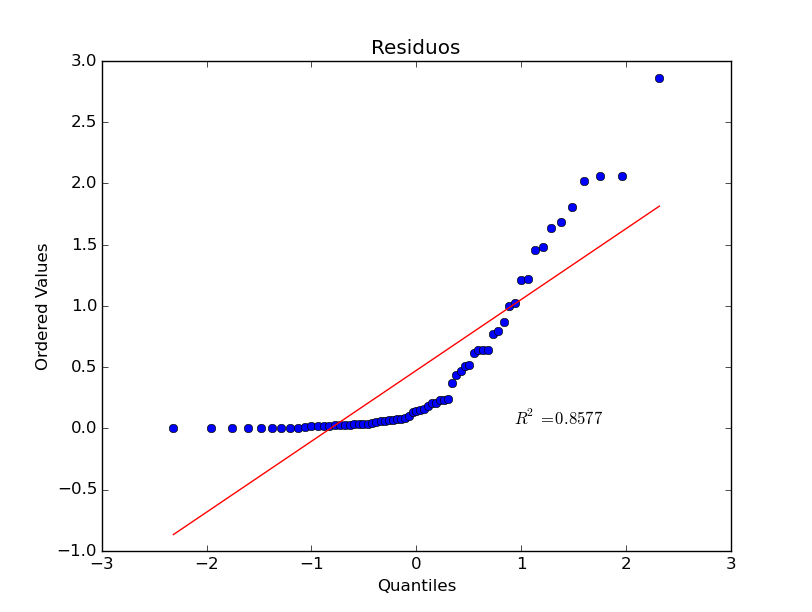
\includegraphics[width=0.55\textwidth]{images/qqplot}
   \caption{Q-Q plot del error de los datos de entrenamiento}
   \label{fig:mesh1}
\end{figure}

Se puede observar por el comportamiento del gráfico, que los datos son próximos a la recta roja, lo que quiere decir que los datos siguen fielmente una distribución normal, traduciéndose en que el residuo del modelo se comporta como una distribución normal. Esto indica que la variables de entradas (input set) y la variable de salida (target) se correlacionan linealmente, tal cual indica la ecuación \eqref{f_rlineal}, pudiendo hacer una regresión con todos los supuestos que esta cumple.

\end{itemize}
\newpage
\subsection{Selección de Atributos}
Utilizando el mismo dataset (\textit{prostate-cancer}) se realiza un estudio sobre seleccionar los atributos/características esenciales, es decir, que afectan más el resultado de la variable que se desea predecir (target). Se realizan dos métodos para analizar el impacto que tiene cada atributo sobre el target, una es mediante FSS en donde se va seleccionando cada atributo, uno por uno, siendo esa variable la mejor en ese momento. Otra es mediante BSS, la cual va eliminando un atributo en cada iteración, siendo ese atributo el que menos influencia tiene en el resultado de la variable target.

\begin{itemize}
\item[a)] FSS parte de un modelo sin atributos (variables) y agrega uno a la vez, eligiendo la mejor localmente. Para este caso la selección de los atributos fue en el orden siguiente:

\begin{table}[!htb]
 \begin{center}
   \begin{tabular}{|c|c|c|c|} \hline
   i & Variable seleccionada & MSE & variables \\ \hline
   1 & Lcavol & 0.876172 &1 \\
   2 & Lweight & 0.752606 &2 \\
   3 & Lbph & 0.748883 &3 \\
   4 & Svi & 0.746635 &4 \\
   5 & Pgg45 & 0.748007 &5 \\
   6 & Lcp & 0.734094 &6 \\
   7 & Age & 0.726706 &7 \\
   8 & Gleason & 0.757237 &8 \\ \hline 
   \end{tabular}
 \end{center}
\end{table}

Donde el número de variables ($\beta_i$) va aumentando ya que el modelo lineal va adquiriendo más características, partiendo desde 1 variable, es decir, una típica función lineal en un plano.\\
En la tabla, las primeras características en escoger son \textit{Lcavol} y \textit{Lweight}, corroborando el análisis anterior hecho con el Z-score de las variables (atributos) en el modelo, por lo que se puede ver que FSS dice que estas dos primeras características son las más relevantes para predecir el target. Se ve como la última característica en ser escogida es \textit{Gleason}, por lo que se puede decir que según FSS esta característica tiene la menor influencia sobre el target.\\

Se realiza un gráfico con los errores de entrenamiento y de test, sobre cada modelo que se construyó con cada selección de las características descritas en la tabla superior. Mostrando a continuación:

\begin{figure}[!htb]
   \centering
   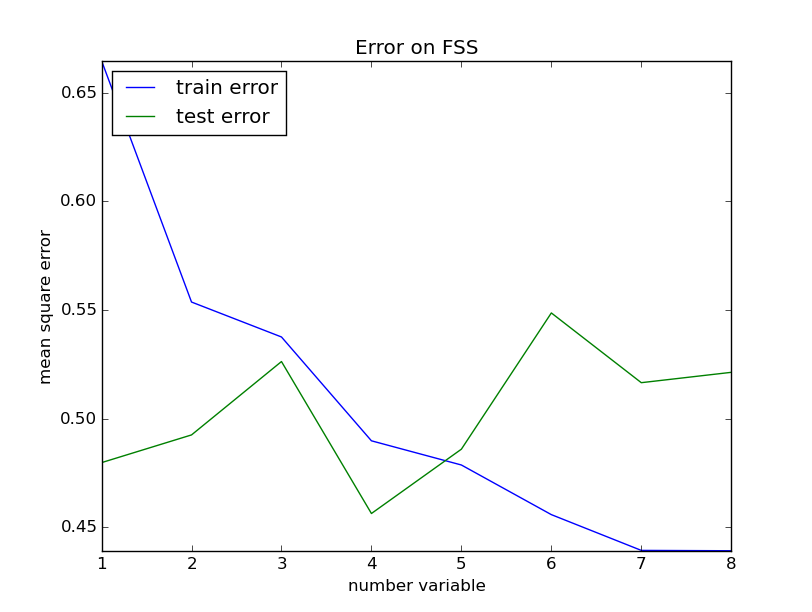
\includegraphics[width=0.55\textwidth]{images/fss}
   \caption{errores en FSS en regresión lineal ordinaria}
   \label{fig:mesh1}
\end{figure}

Como el error de entrenamiento disminuye a medida que se escogen más variables, esto se debe a que el algoritmo FSS funciona de esta manera, trabajando sobre el training set y escogiendo lo que es más óptimo para este, donde mientras más variables se seleccionan más se puede predecir del target, ya que el error va disminuyendo. \\

Para el caso del error de testing, este varía aleatoriamente, ya que no existen métodos para predecir este error, por lo que las decisiones que va tomando FSS no entregan información sobre el error de test, sino que realiza operaciones sobre el training set, esperando que estas afecten al test set.\\
En el gráfico anterior, en el caso que el número de variables se acerca a la cantidad máxima del modelo, el error de entrenamiento disminuye, incluso llegando a ser menor que el error de prueba. Este caso se conoce como \textit{overfitting}, donde el modelo se sobre-ajusta a los datos de entrenamiento, prediciendo que el error disminuye, siendo que en verdad este se mantiene igual.

\item[b)] BSS parte de un modelo completo (todas las características), eliminando una característica a la vez. Para este caso, el orden de eliminar cada atributo fue el siguiente:

\begin{table}[!htb]
 \begin{center}
   \begin{tabular}{|c|c|c|c|} \hline
   i & Variable seleccionada & MSE & variables \\ \hline
   1 & Gleason & 0.726706 &8 \\
   2 & Age & 0.734094 &7 \\
   3 & Lcp & 0.748007 &6 \\
   4 & Pgg45 & 0.746635 &5 \\
   5 & Svi & 0.748883 &4 \\
   6 & Lbph & 0.752606 &3 \\
   7 & Lweight & 0.876172 &2 \\
   8 & Lcavol & 1.795596 &1 \\ \hline 
   \end{tabular}
 \end{center}
\end{table}
Para esta tabla el número de variables (última columna) son las variables presentes en el modelo, es por esto que va disminuyendo, ya que en cada iteración se va eliminando la peor.\\
Se puede ver como la primera variable en ser eliminada fue la característica \textit{Gleason}, análogo al caso de FSS donde esa fue la última característica en ser seleccionada, por lo que se puede decir que según BSS esta característica es la que menos peso tiene al predecir la variable target. Se observa como las últimas características en ser eliminadas son \textit{Lcavol} y \textit{Lweight}, análogo al caso de FSS y entregando más argumentos a favor de que estas son las características más relevantes del modelo.\\

Se presentan los errores entrenamiento y prueba para cada modelo formado con las características asociadas en la eliminación:

\begin{figure}[!htb]
   \centering
   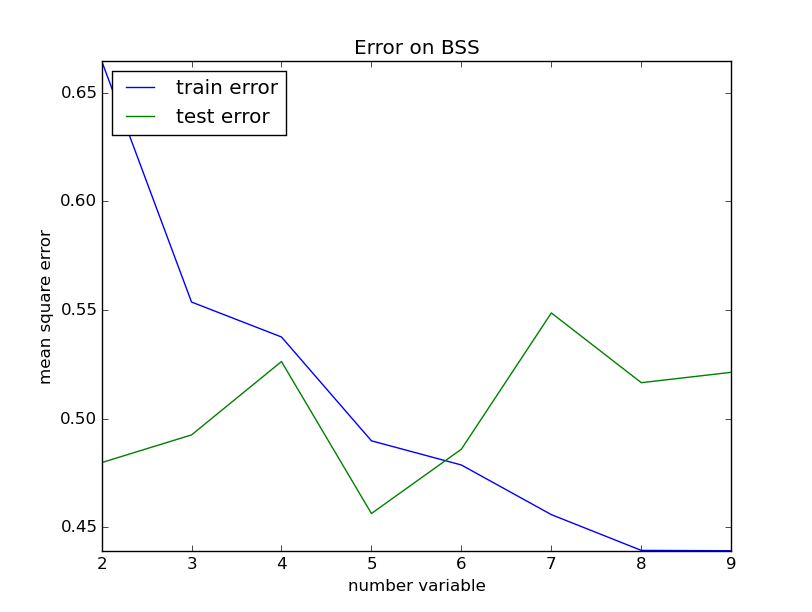
\includegraphics[width=0.55\textwidth]{images/bss}
   \caption{error BSS en regresión lineal ordinaria}
   \label{fig:mesh1}
\end{figure}

Gráfico similar al caso del algoritmo FSS, esto ocurre ya que estos algoritmos trabajan sobre el training set y uno es análogo a otro, ya que ambos llegan al mismo resultado, es decir, al mismo orden de importancia de las características. \\
A medida que se le agregan más características al modelo, este se ajusta más al training set, por lo que existe una precisión mayor al predecir el target en el training set. Para el test set no es posible predecir o disminuir este error con la selección.\\
\end{itemize}

\subsection{Regularización}

En esta parte del informe se tratará el tema de la regularización, en donde se castigan los coeficientes altos del modelo lineal, regularizando estos y dándoles un límite de valor para tomar y ver como afecta esto al modelo. Para eso se harán distintas comparaciones entre los errores de test y entrenamiento, para distintos algoritmos de aprendizaje donde cada uno tiene un método de regularización diferente, incluyendo diferentes rangos en la regularización.
\begin{itemize}

\item[a)] En primer lugar, se estudia la regularización del método de ''\textit{Ridge Regression}'' el cual regulariza los atributos o variables, para obtener un modelo lineal más preciso y así poder analizar la data de mejor forma y obtener comparaciones entre estas variables.\\
En el código entregado, en la tercera línea se puede observar que se elimina la columna \textit{ intercept} con el método \textit{drop()}, puesto que ya no se necesita, ya que la regularización es sobre los atributos/características del modelo y el intercepto no es modificado.\\
Además, en la novena línea se ejecuta el método de Ridge a través de la factorización svd, con el parámetro \textit{fit intercept} asignado como \textit{True}, puesto que como la columna fue eliminada, el mismo método se encarga de calcular el intercepto.\\

A continuación, se presenta el gráfico de la regularización:\\

\begin{figure}[!htb]
   \centering
   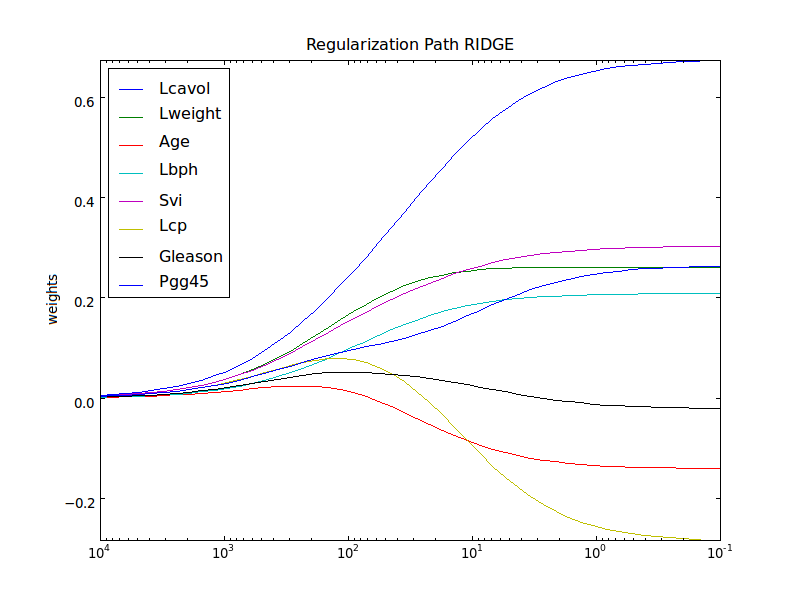
\includegraphics[width=0.55\textwidth]{images/regularization_ridge}
   \caption{Gráfico de regularización de Ridge.}
   \label{ridge}
\end{figure}

El gráfico representa el peso que tiene cada variable o característica (eje y) en el modelo general por cada alpha (eje x) estudiado en el rango [$10^4$,$10^{-1}$]. La forma del gráfico se atribuye a la restricción cuadrática que presenta la regresión:

\begin{equation} \label{ridge}
\sum_{i=1}^I \beta_i^2 \leq s
\end{equation}

Se puede observar del gráfico que las características que poseen un peso superior a las demás características son \textit{Lcavol} y \textit{Lweight}, puesto que al ir disminuyendo el valor de alpha, los pesos de estas variables aumentan más que las otras. También se puede ver que \textit{svi} empieza a tener más peso que la variable \textit{Lweight} solamente al disminuir el alpha a un valor inferior a $10^{-1}$. Esto apoya las afirmaciones anteriores de los métodos FSS, BSS y Z-score con un nivel de significancia del 5\%, obteniendo los mismos resultados, es decir, las variables \textit{Lcavol} y \textit{Lweight} poseen más incidencia en la decisión (target).


\item[b)] Por otro lado, se puede hacer el mismo análisis para la regularización con el método de ''\textit{Lasso}'', regularizando los atributos de una manera más estricta que ''\textit{Ridge}'', ya que tiene una penalización más alta para los atributos, siendo más riguroso a la hora de decidir cuál característica tendrá más peso en el modelo.\\

Para esto se obtiene el siguiente gráfico:
\begin{figure}[!htb]
   \centering
   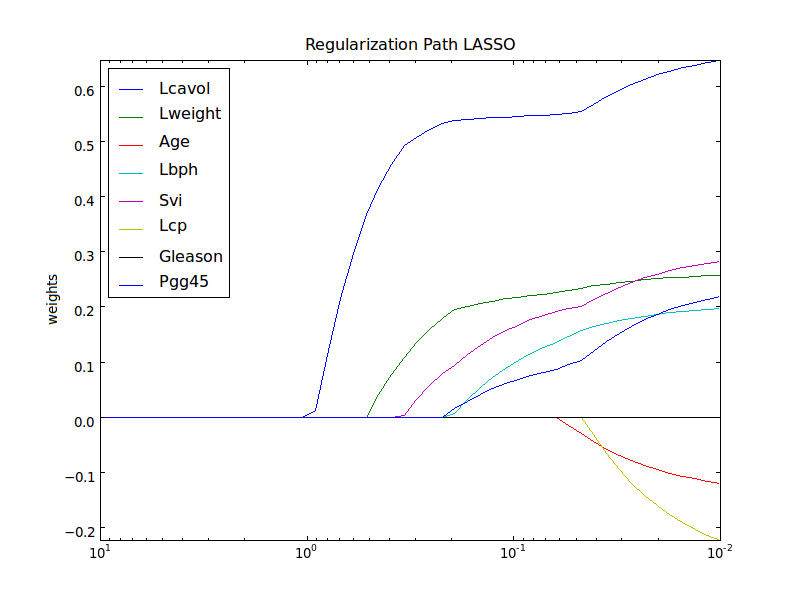
\includegraphics[width=0.55\textwidth]{images/regularization_lasso}
   \caption{Gráfico de regularización de Lasso}
   \label{lasso}
\end{figure}

El gráfico representa el peso que tiene cada variable o característica (eje y) en el modelo general por cada alpha (eje x) estudiado en el rango [$10^1$,$10^{-2}$]. La forma del gráfico se atribuye a la restricción lineal siguiente: \\

\begin{equation}
\sum_{i=1}^I |\beta| \leq s
\end{equation}

Se puede observar del gráfico, que posee una forma mucho menos ''suave'' que con el método de \textit{Ridge}, incluso llevando los pesos de cada variable a cero luego de aumentar el valor de alpha más allá de $10^0$. Esto concuerda con lo esperado, puesto que se sabe de antemano que \textit{Lasso} posee un nivel de penalización mucho más riguroso, y por lo tanto, a medida que los valores de alpha disminuyen la diferencia entre los pesos de las variables es más notoria.\\

\item[c)] Para este caso se visualiza gráficamente cómo se relaciona el error de prueba y de entrenamiento con la penalización (alpha), mostrando a continuación:\\

\begin{figure}[!htb]
   \centering
   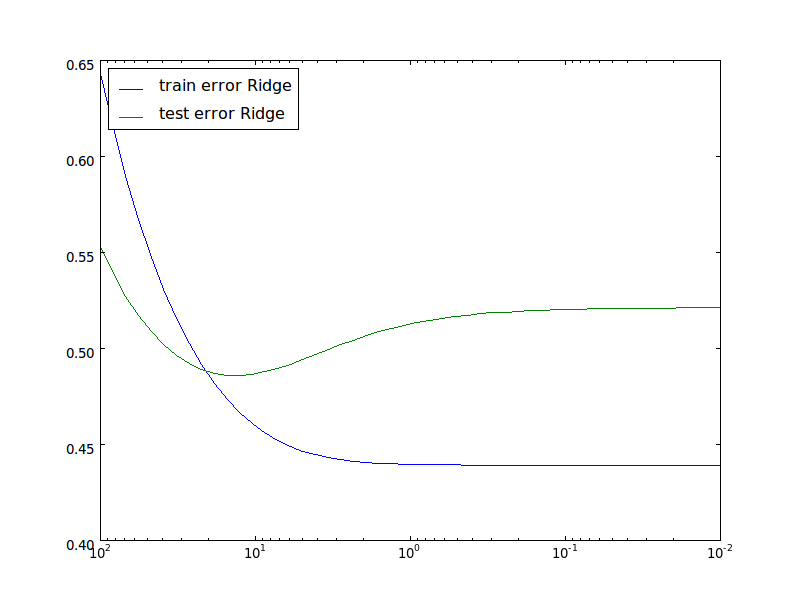
\includegraphics[width=0.55\textwidth]{images/alphas_ridge}
   \caption{Errores en modelo de Ridge para distintos alphas.}
   \label{err:ridge}
\end{figure}

\newpage

Si se realiza un análisis en conjunto con la ecuación de Ridge ($\beta^{ridge}$), se observa que para alphas pequeños ($\alpha \sim 0$) la penalización es baja, por lo tanto, los valores de $\beta_i$ no están tan limitados, obteniendo valores similares a las del modelo de regresión lineal ordinaria. A medida que aumenta el valor de alpha, y con esto la penalización, los valores de $\beta_i$ se ven más restringidos, traduciéndose a una ecuación en donde las características no van a tener tanta influencia sobre el target, dependiendo en gran medida del intercepto.

La forma cuadrática del gráfico nuevamente se atribuye a la ecuación \eqref{ridge}. Este método de Ridge tiene un objetivo similar que los métodos de selección de características (FSS y BSS), pero en lugar de eliminar las características del modelo estas son ''amortiguadas'' asignándoles un coeficiente (peso) bastante bajo.\\
Se puede observar además, que para este caso, un alpha apropiado en el modelo de Ridge, es mejor que el de mínimos cuadrados, ya que el test error disminuye en una fracción del gráfico. Esto es tan sólo analizable desde el ''exterior'' del algoritmo de aprendizaje, ya que este no tiene acceso al test data.


\item[d)] Análogo al caso anterior, se ve como afecta la penalización de la variable \textit{alpha} para los distintos atributos:

\begin{figure}[H]
   \centering
   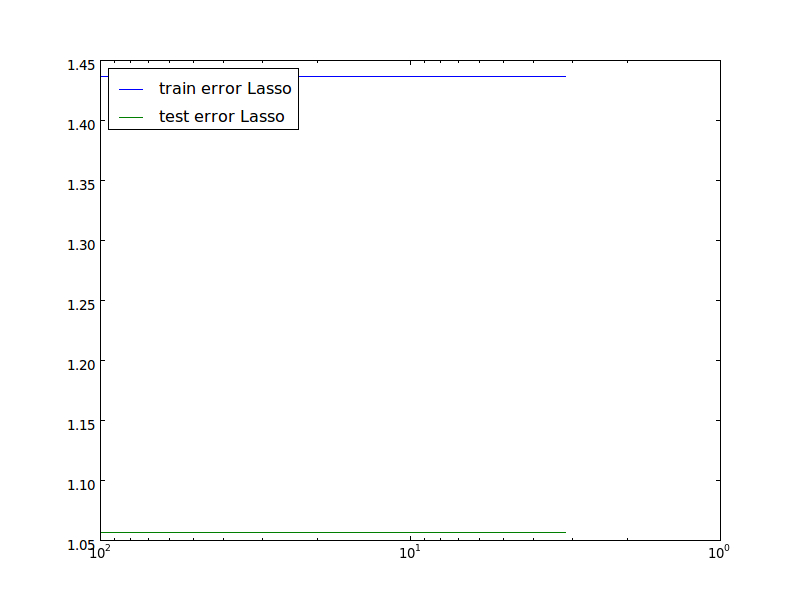
\includegraphics[width=0.55\textwidth]{images/alphas_lasso}
   \caption{Errores en modelo de Lasso para distintos alphas.}
   \label{err:lasso}
\end{figure}

En contraste a la ecuación de Lasso se conoce que esta es bastante restrictiva con los coeficientes ($\beta_i$). Esto es visualizado en el gráfico, ya que para los valores de alpha que se presentan los coeficientes ya han sido asignados a cero (ver gráfico \ref{lasso}), por lo que los errores que se presentan son de un modelo sin variables, es decir, un modelo constante, y de ahí la forma del gráfico. Se puede ver que para valores pequeños de alpha estos ya generan que el modelo no tenga variables ($\beta_i = 0 \ \ \forall i$). De esto se desprende que el modelo a utilizar va a depender del training set, es decir, si se desea nivelar el peso de ciertas características de una forma más fuerte que Ridge, es conveniente usar Lasso.


\item[e)] Para conocer qué valor de \textit{alpha} es el óptimo en los distintos métodos presentados (Lasso y Ridge). Se utiliza la técnica \textit{cross-validation} con el fin de probar distintos alphas y medir el error con los \textit{k-folds}, para luego determinar el alpha con menor error cuadrático medio de todos los cross-validation.\\

Para los distintos modelos se obtuvieron los siguientes resultados:

\begin{itemize}

\item Método de Ridge: $\hat{\alpha} = 2.33$, con un error de mse(cv): $0.75$
\item Método de Lasso: $\hat{\alpha} = 0.10$, con un error de mse(cv): $0.87$

\end{itemize}

Al comparar ambos métodos, es fácil visualizar que el método de Ridge posee un error cuadrático medio menor que el de Lasso, esto nos quiere decir que el modelo, con su alpha correspondiente, más seguro sería el de Ridge.





\end{itemize}

\subsection{Predicción de utilidades de películas}

En esta parte del informe, se trabaja con un dataset que contiene datos sobre películas \cite{joshi2010movie}, con el objetivo de hacer un estudio sobre estas y poder predecir las utilidades que se obtendrán del estreno de cada una en USA.

\begin{itemize}

\item[a)] En primer lugar, se cuenta con una matriz de gran tamaño, la cual contiene muchos datos nulos, por lo que la estructura en la que se presenta esta matriz es en un formato sparse (disperso), es decir, los valores no nulos se encuentran alejados unos de otros, presentándose en un formato en el cual se guardan los datos no nulos de la siguiente manera: \textit{(indice i, indice j, valor)}. Mantener este formato es de gran utilidad, ya que no solo ahorra espacio en el disco, sino que también provee eficiencia en operaciones aritméticas y producto matriz vector. \\
Se conoce que los modelos de regresión lineal utilizan operaciones matriz vector, las cuales son costosas computacionalmente y dificultarían de gran manera el estudio de los datos a medida que el tamaño de estos aumenta, por lo que mantener el formato $sparse$ es necesario.

\item[b)] Se construye un modelo lineal para obtener el coeficiente de determinación sobre el conjunto de pruebas. Para esto se analizan dos datasets similares, donde uno posee más características que otro. Al dataset con menos características lo llamaremos $X$ y al otro $X'$.
Se comienza el análisis probando con un modelo de regresión lineal ordinaria, para el cual se calcula el score asociado, es decir, que tan bueno es el modelo en su aprendizaje (valor de 0 a 1).

Se obtienen los siguiente resultados para cada dataset:

\begin{itemize}

\item Para $X$: Score: $0.5903$
\item Para $X'$: Score: $0.2062$ 

\end{itemize}

Con estos valores se obtiene un primer acercamiento a los coeficientes de determinación que se desea alcanzar (0.75) y como se puede observar, no se obtiene un score suficiente para ningún dataset. También se puede observar que en $X$ se obtiene un score más alto, por lo que el input set ($\chi$) tiene un mejor comportamiento para la regresión lineal ordinaria en este caso.\\

Luego de este acercamiento, se piensa que como X tiene un mayor score, es posible que si se le remueven más características al dataset, se obtenga un mejor ajuste, traduciéndose a un mejor score. Para esto se aplica el método FSS realizado anteriormente, el cual no es logrado computacionalmente debido a que este método posee un bucle \textit{for()}, el cual se repite $I$ veces, donde $I$ es el número de características del modelo ($> 10^5$), por lo que se excede la capacidad límite soportada.

Se sabe por lo visto anteriormente, que los métodos de regularización realizan un ajuste a las características de manera de no eliminarlas por completo de la función lineal.

Aplicando el método de Ridge se obtienen los siguientes coeficientes de determinación ($R$):

\begin{itemize}

\item Para $X$: $R=0.5918$, con $alpha = 1676.833$
\item Para $X'$: $R=a$, con $alpha = XX$

\end{itemize}

Donde además se construye el siguiente gráfico comparativo para $X$:

\begin{figure}[!htb]
   \centering
   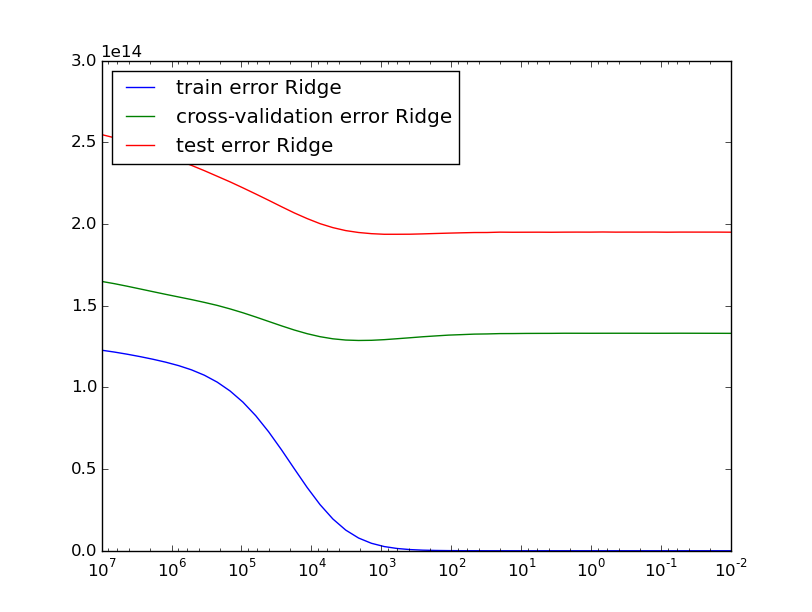
\includegraphics[width=0.55\textwidth]{images/comparacion_ridge}
   \caption{Errores en modelo de Ridge para distintos alphas.}
   \label{err:lasso}
\end{figure}

\begin{figure}[!htb]
   \centering
   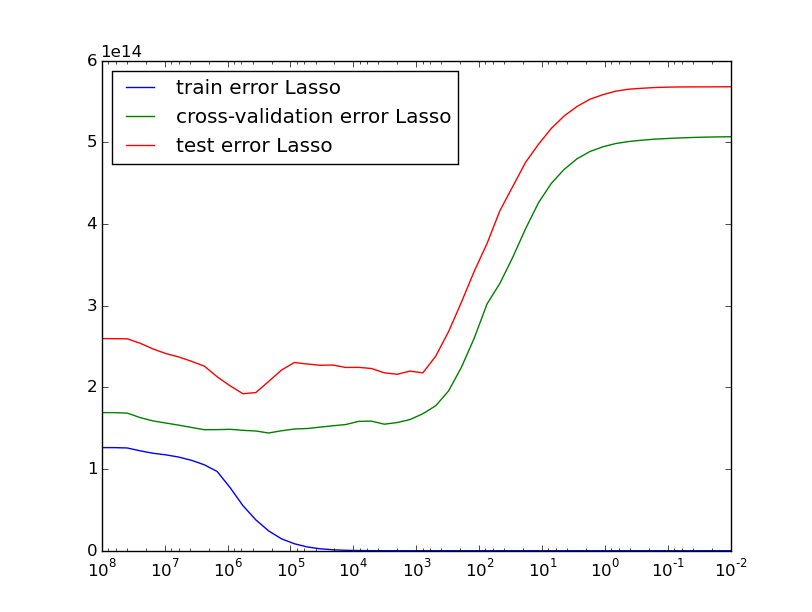
\includegraphics[width=0.55\textwidth]{images/comparacion_lasso}
   \caption{Errores en modelo de Lasso para distintos alphas.}
   \label{err:lasso}
\end{figure}

Donde se observa claramente, que para distintos alpha's, no es posible disminuir el error de validación, ya que a medida que disminuye el alpha, el error se aproxima a mínimos cuadrados, y a medida que aumenta, el error lo hace también. Por lo que el óptimo encontrado con $alpha = 1676.833$ es el mejor para el modelo de Ridge en el dataset $X$.


\end{itemize}
 
\section*{Anexo}

\noindent Códigos adjuntados en archivos .py


\bibliographystyle{abbrv}
\bibliography{master}


\end{document}
